\documentclass[twocolumn,10pt]{article}
\usepackage[utf8]{inputenc}
\usepackage{amsmath}
\usepackage{graphicx}
\usepackage[margin=0.75in]{geometry}
\usepackage{subfigure}

\title{Implementing Nullifiers in a One-Time Note Sharing DApp: Preventing Double-Spending}
\author{Edgar Blumenthal, Justus Krebs, Hanna Lichtenberg}
\date{}

\begin{document}

\maketitle

\section*{Project Goal and Objectives}
The primary goal of this miniproject was to solve the issue of double spending in decentralized applications (DApps) by using cryptographic nullifiers. Double spending, where a digital asset is used more than once, poses a significant challenge in various scenarios such as voting systems or tumblers of digital currencies, such as Tornado Cash. Our objective was to implement a nullifier mechanism within a DApp to prevent double spending of a digital asset.

\section*{Our Idea}
To meet this objective, we developed a proof-of-concept DApp designed for secure one-time note sharing. This application uses cryptographic nullifiers to guarantee that each note can be read only once, thus solving an instance of the double spending problem in the form of reading the same note twice.

\section*{Implementation}
The project involved several key steps: (1) We used a SHA256 hash function to create a unique nullifier for each note by combining the note itself and the unix time, ensuring each nullifier is distinct and anonymous, thus preserving user privacy. The note is then encrypted using the nullifier as the secret key. (2) Both the note and the nullifier are then send to a smart contract on the Ethereum testnet blockchain to create a mapping between note and nullifier. Upon retrieval the smart contract verifies if a nullifier has already been used before granting access to the associated note. (3) A user-friendly DApp was developed to allow users to create, encrypt, store, and retrieve notes using nullifiers. A sequence diagram of the above described implementation and a screenshot of the DApp can be found in the appendix \ref{fig:version1} and \ref{fig:web3} .

\section*{Challenges and Learnings}
The project demonstrated the feasability of using cryptographic nullifiers to prevent double spending using the example of one time note sharing.
When evaluating the outcome of our project, we encountered several challenges that provided valuable learning opportunities:
\begin{itemize}
    \item \textbf{Security Concerns}: One of the significant challenges was ensuring that the nullifier and the encrypted note, once stored on the blockchain, could not be easily decrypted by unauthorized parties. We identified a potential vulnerability in our approach, which requires storing both the encrypted note and the nullifier on the blockchain to create the mapping and check against used nullifiers. This exposes the data to unauthorized parties, as someone knowing the cipher could potentially use the stored encrypted data and the nullifier to decrypt the note. We therefore proposed the use of a key derivation function (KDF) to derive the nullifer and a secret encryption key from a sharable secret, mitigating the need to store the encryption key on the blockchain along the note. This new approach can be seen in the second sequence diagram \ref{fig:version2}.
    \item \textbf{Blockchain Limitations}: The immutable append only nature of the blockchain presented a challenge for our DApp. While our implementation prevented double reading from the frontend, the encrypted data remained accessible on the blockchain. This highlighted the need for further innovation in managing data lifecycle within blockchain systems.
    \item \textbf{Trust and Censorship}: When comparing our decentralized approach to traditional centralized systems, we noted significant drawbacks of the latter. This includes the need of complete trust in the provider to not delete the note or alter the nullifier. Centralized systems rely on the provider to manage data integrity and access, which can be a single point of failure and a risk for users. In contrast by using the Ethereum blockchain we can rely on all participants to store and execute the business logic i.e. the smart contract.
\end{itemize}

\section*{Conclusion}
The approach we implemented has generally worked well, particularly from the frontend and DApp perspective, successfully preventing double spending within the user interface. However, to ensure true one-time readability on the blockchain itself, we suspect that the use of zero knowledge proofs might be advantageous.

\onecolumn

\section*{Appendix}

\begin{figure}[h]
    \centering
    \begin{minipage}[b]{0.48\textwidth}
        \centering
        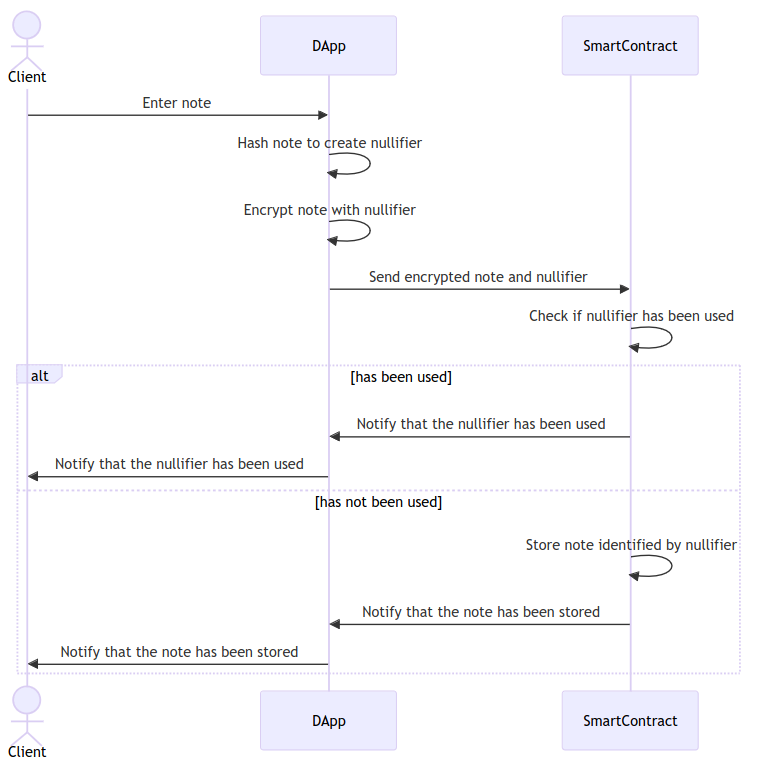
\includegraphics[width=\linewidth]{./figures/version1.png}
        \caption{Version 1}
        \label{fig:version1}
    \end{minipage}
    \hfill
    \begin{minipage}[b]{0.48\textwidth}
        \centering
        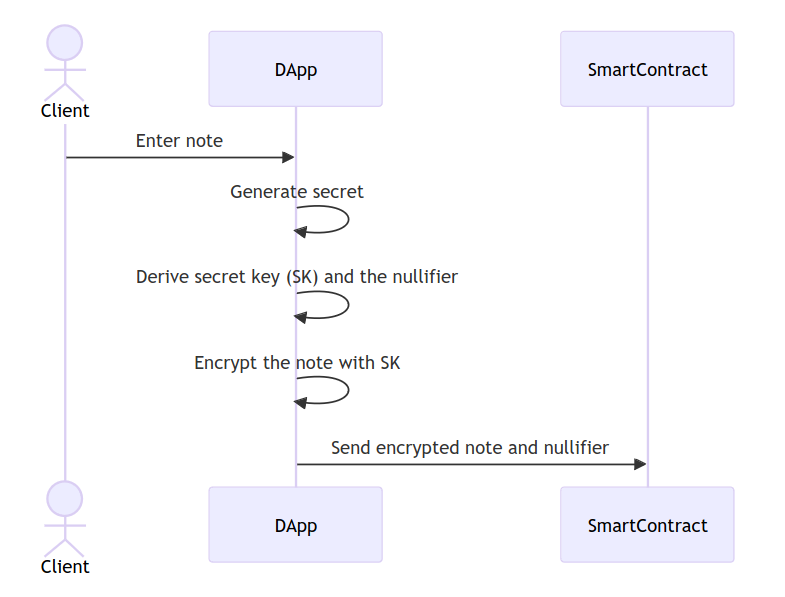
\includegraphics[width=\linewidth]{./figures/version2.png}
        \caption{Version 2}
        \label{fig:version2}
    \end{minipage}
    \caption{Comparison of Version 1 and Version 2}
    \label{fig:versions_comparison}
\end{figure}
\begin{figure}[!htb]
    \centering
    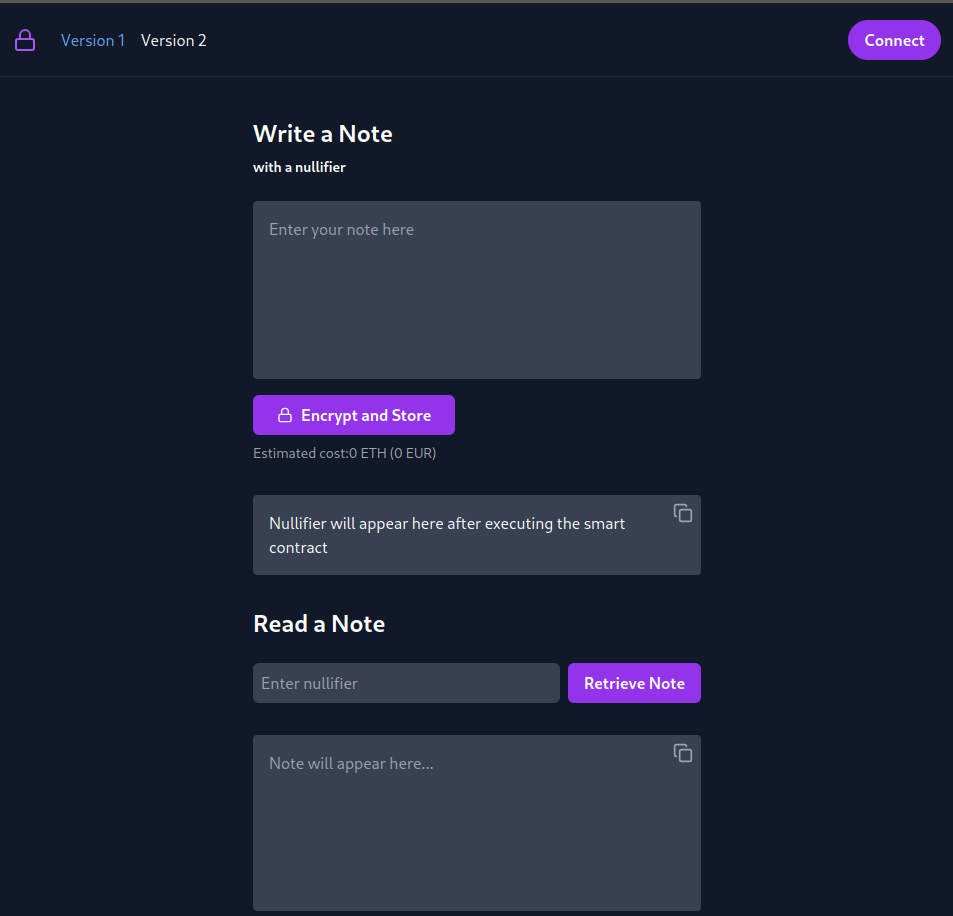
\includegraphics[width=0.6\textwidth]{./figures/web3.png}
    \caption{Decentralized Application UI}
    \label{fig:web3}
\end{figure}

\end{document}

